\documentclass[twoside]{report}
\usepackage[utf8]{inputenc}
\usepackage{VassorTitle}
\usepackage[super]{nth}
\usepackage{lettrine}
\usepackage{xstring}
\usepackage{todonotes}
\usepackage{graphicx}
\usepackage{tikz}
\usepackage{csquotes}
\usepackage{pdflscape}


\institution{École polytechnique fédérale de Lausanne}
\project{\nth{1} semester report --- HUM-428}
\supervisor{Pr.~\textsc{Vinck}}


%\renewcommand\paragraph[1]
%{
%	\lettrine{\StrLeft #1 {1}}{\StrGobbleLeft #1 {1}}
%}
% TODO : Lettrine paragraphe

\graphicspath{{figures/}}

% Document description
\title{Proposal for a methodology of start-up analysis}
\author{Giulia \textsc{Ferrari}\\Martin \textsc{Vassor}}

% Beginning document
\begin{document}
\maketitle
\begin{abstract}
	\paragraph{}
	This report is made for the HUM-428(a) course entitled \emph{Sciences,~technology~and~society}, told by Pr.~\textsc{Vinck} with Richard~\textsc{Marion} and Alexandre~\textsc{Camus} as lecturer assistants at the \textsc{École Polytechnique Fédérale de Lausanne}. Its goal is to conclude the fall semester lectures and provide a base for spring semester work. 

	For this purpose, it first sums up the knowledge acquired during the semester, making a link between the theoretical concepts and the interventions of external lecturers. Then, it proposes a methodology for the study case we'll do in the forthcoming semester.
\end{abstract}
\tableofcontents
%\listoffigures
%\listoftables
\chapter*{Introduction}
\paragraph{}
Incertitude is a concept with a transversal character. Although we are all aware of its existence, we do not comprehend its pregnance in every activity or project that we undertake. We seem to think that uncertainty concerns future events and expectations, but few men of experience actually understand how it shapes the whole environment in which we live. As middle school students who had to make a choice between different kinds of high schools we all were uncertain of how our future would be should we choose one instead of another, but as entrepreneurs who make a living out of the success of their businesses incertitude in the form of market reception, product definition and feasibility represents a very real issue. \enquote{In some cases there might exist certain methods – statistical or not – that allow us to measure risks to a certain degree, however in industries such as nanotechnologies uncertainty remains a vague concept, because people don’t analyze the consequences of their actions, thus they do not possess that knowledge that would otherwise help them increasing the occurrence of positive results.}\cite{chalas_comment_2009}
\paragraph{}
The goal of this report is to provide a start-up with the means to decrease risks and overall uncertainty for their future activities. That of the start-ups is undoubtedly a minefield, as incertitude is a particularly sensitive subject with respect to innovation, which notably produces a fair amount of unknown. Furthermore, the start-up that will be taken as a reference throughout the report – SqeedTime – belongs to the industry sector of mobile applications, whose innovative character is particularly pronounced. This leads us to estimate that uncertainty constitutes a major issue for this recently founded enterprise. Hence, in order to reduce it, determining its influence on the every-day activities and future events is of the essence.
\paragraph{}
The structure of the report is such that it evidences the steps that we took to formulate a plan for the flanking activity of SqeedTime that will take place over the next semester. Chapter \ref{ch:knowledge} recapitulates the main notions that we learned from the experiences of four different start-ups – Hidacs, Future Instruments, GlobalNeonat, Artanim Interactive – whose founders/initiators were invited in the course of the first semester. Chapter \ref{ch:description} introduces the start-up in exam, putting emphasis on its innovative product, organization and meaningful facts that have been accrued since its foundation a year ago. A preliminary estimation of its level of uncertainty can be done studying the activity sector and the experiences of similar start-ups that currently find themselves at a more advanced stage. Thus, chapter \ref{ch:kinds} describes the main sources of incertitude that pertain to mobile applications and provides recommendations to new entrepreneurs that want to embark on the same business, in order for them to take as many risk-reducing measures as possible at the very beginning. With the information gathered so far, it is therefore possible to formulate a working methodology that can be applied in the second semester when working with the start-up members, as it is illustrated in chapter \ref{ch:method}. 
\chapter{Acquired knowledge}
\label{ch:knowledge}
\section{External lecturers}
\begin{table}[h]
	\begin{tabular}{|ccp{5cm}|}
		\hline
		\textsc{Start-up} & \textsc{Innovator} & \textsc{Product} \\ \hline
		Hidacs & Patrick \textsc{Marmaroli} & High end directional loudspeaker that diffuses light and music locally. \\
		Future Instruments & Alain \textsc{Crevoisier} & Technology that transforms any flat surface into a tactile interface. \\
		GlobalNeonat & Benjamin \textsc{Rime} & Incubator made of PCMs  for developing countries.\\
		Artanim Interactive & Alain \textsc{Renaud} & Series of products based on innovative algorithms in the domain of motion capture. \\
		\hline
	\end{tabular}
	\caption{Start-ups and their products that were examined during the sessions in class.}
	\label{tab:lecturers}
\end{table}
\section{The notion of uncertainty}
\paragraph{}
Uncertainty is a notion that concerns every facet of modernity. At times it may seem inconsequential, but it could not appear more evident in the sessions during which guests spoke about their innovative ideas and start-ups (see table~\ref{tab:lecturers}~p.\pageref{tab:lecturers}). 
\paragraph{}
They have been invited to recount their experiences to the class, but on a deeper level they were actually talking about the numerous occasions in which they concretely came face-to-face with uncertainty. This is a common occurrence especially in the case of start-ups, whose essential nature is aptly captured by \textsc{Ries} (\cite{ries_what_2010}). He defines a start-up as a \begin{quote}\enquote{human institution designed to deliver a new product or service under conditions of extreme uncertainty.}\end{quote}
	\paragraph{}
	It is foremost a human enterprise because, like in any other company, the value creation is located in the people who work together to create a product out of the original idea, creative employees are hired and then must be coordinated to deliver results.  Secondly, a start-up aims to uncover a new source of value for customers, thus proposing a new product to them. The question of innovation is more delicate, since we find that even the most radical new inventions build upon previous technology. Even if we are used to think of a new product whenever innovation is mentioned, a lot of start-ups don't innovate at all in the product dimension but they base their work on repurposing an existing technology for a new use (such is the case of GlobalNeonat, that found another application for phase-change materials, integrating it into a new kind of incubator), devising a new business model or simply locating an existing product or service in an unexplored geographical area. 
	\paragraph{}
However, what really distinguishes start-ups from the rest of the companies – small and large alike – is the context in which they work: one of extreme uncertainty. As \textsc{Ries} (\cite{ries_what_2010}) explains : \enquote{start-ups are designed for the situations that cannot be modeled, are not clear-cut, and where the risk is not necessarily large – it's just not yet known}. This applies to factors that can be either external – such as the existence of a market and the propensity of potential financiers to invest in the project – or internal – such as the actual feasibility of the invention, the way to conduct the development process, the amount of time and resources that should be accounted for. When success is not guaranteed, there is always a measure of risk involved and it is clear that a company for which uncertainty is not the main concern does not belong to the \emph{start-up domain}.
	\paragraph{}
	This is also the reason why common management best practices do not apply to start-ups. For instance, the common entrepreneur is prone to think that when a new project is on track, on time and on budget it is well-managed and will lead to success. This is not true in the start-up case, since if an ardent innovator fails to understand that he is building something that in the end will not interest any kind of customer, even a perfectly conducted project will be wasted effort. This was precisely the case of Future Instruments. The founder, Mr. \textsc{Crevoisier}, is an ardent fan of electronic music and he devoted ten years of his life to find a way to make his idea a reality. The new technology was born out of and built on the basis of his own needs; in 2007, with the construction of the first prototype, the product was ready to be launched on the market. However, potential investors, though believing the idea held merit, responded with a rejection, as a real market – beside the inventor – didn't exist. For this same reason, Future Instruments also represents a manifest example of the so-called \emph{innovator's four pathologies}, at least where lack of criticism acceptance and definition of pathway and market are concerned. 
	\paragraph{}
	As \textsc{\textsc{Ries}} wrote in \cite{ries_is_2010} : 
	\begin{quote}
		\enquote{
		All entrepreneurs face the same fundamental challenges:
		\begin{itemize}
			\item How do we know if we're making progress?
			\item How do we know if customers will want the product we are building?
			\item And, if they do, how do we know what kind of value we can create with it? 
		\end{itemize}}
	\end{quote}
	But because every start-up strives to become an institution and build a sustainable business, answering these questions requires progressively acquired learning and a specifically tailored kind of accounting. This can be achieved through the coordination of many different people, who must work together to find the answers. In fact, one of the aspects which the four start-ups in exam have in common is precisely teamwork. The enterprises might have originated either from a foundation spin-off, a master project in university, the university laboratory or simply from the ambitious idea of a man, but they ultimately grew to include more people who provide their expertise in various fields as well as valuable advice. 
	\paragraph{}
	When analyzing the four different cases of start-ups, we have been able to realize that there exist as many differences as few commonalities between them. However, the background, experiences and ideas may be very different, but the overall uncertainty concerns the same aspects:
	\begin{itemize}
		\item market and clients;
		\item product and/or project;
		\item technical feasibility.
	\end{itemize}
	\paragraph{}
	In terms of venture financing, these issues are common in enterprises that are in the \emph{early stage} of their development cycle, which comprehends two consecutive phases: 
	\begin{enumerate}
		\item \emph{the seed stage:} the entrepreneur focuses on fundamental R\&D activities; in the process, he inevitably faces some elementary uncertainties that are also the highest throughout all the life-cycle of the enterprise because at this point both the market acceptance and the product technical feasibility must be evaluated;
		\item \emph{the start-up stage:} once prototypes have been assembled and tests on the product and the market have been conducted, the entrepreneur attempts to commercialize his idea; the risks and the uncertainty are partially mitigated by the preliminary tests, while tasks start becoming numerous and complex, thus the innovator starts hiring additional staff to complement missing expertise. In this manner, he is also alleviating risks regarding the management quality \cite{eckermann_venture_2006}.
	\end{enumerate}
	In addition to this classification, Start-up Commons gathered information from many start-ups all over the world and simplified it into a framework (see fig. \ref{fig:framework} p.\pageref{fig:framework}) that aims to show how innovators usually develop both their ideas and a committed founding team into a real growing business that captures the value being created (\cite{commons_startup_2015}).
	\begin{landscape}
		\begin{figure}
			\begin{center}
				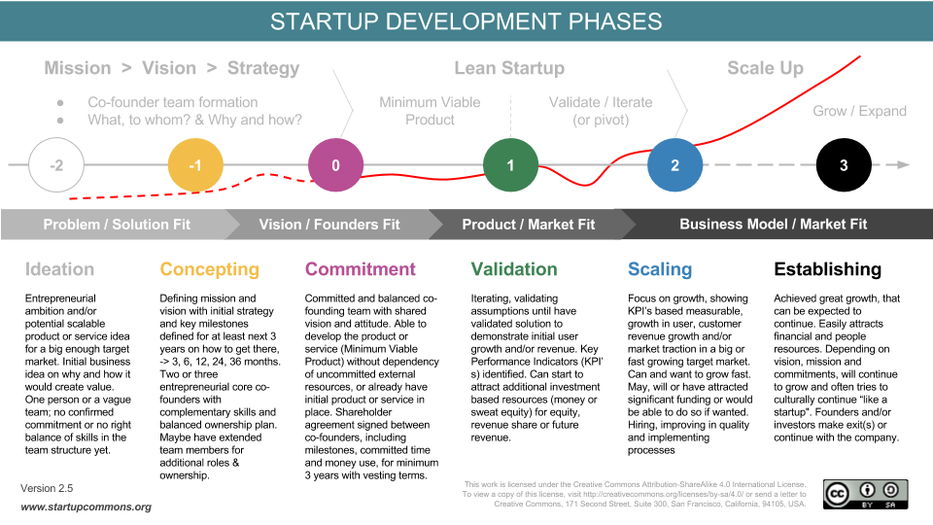
\includegraphics[width=\linewidth]{development_phases.png}
				\caption{Start-up development phases \cite{commons_startup_2015}.}
				\label{fig:framework}
			\end{center}
		\end{figure}
	\end{landscape}
	\paragraph{}
	As far as the examined four start-ups are concerned, all of them experience a certain level of uncertainty related to market. It can be connected to the definition of either the clients or the existing clients' needs (in the case of Hidacs), but it still probably represents the main concern for every newly-formed enterprise. Besides, if a client base existed for every single innovative idea, we would observe so many more start-ups transforming into successful businesses. 
	We have been able to observe that usually the definition of a market is strongly correlated to the start-up's efforts in gathering feedbacks on the targeted clients' acceptance of the product.
	\begin{figure}
		\begin{center}
			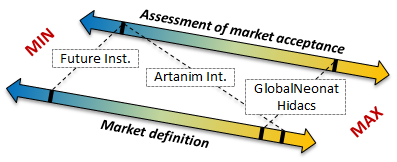
\includegraphics{position.png}
			\caption{How the four start-ups in exam position themselves in terms of market definition and gathering of feedback on market acceptance activities.}
			\label{fig:position}
		\end{center}
	\end{figure}
	As fig. \ref{fig:position} p.~\pageref{fig:position} shows, Future Instruments has major problems in this regard because of Mr. \textsc{Crevoisier}'s lack of sufficient consideration of the customers' needs and wants in the first phase of his start-up. Consequently, he found himself in the disagreeable position of having spent a major part of his life on assertively developing a product whose customers' (still) didn't exist and of having to rapidly find another market segment to target. On the other extreme we find Hidacs and GlobalNeonat, whose client base was already clearly defined before the actual development of the product. Mr. \textsc{Marmaroli} admits to facing market uncertainty every day, but this is due to the difficulty in understanding more the clients' needs when dealing with a customizable product than their identity, which was already known to the Metamedia Center. The same applies to GlobalNeonat, whose main concern was evaluating the market's reception. To solve this issue, Mr. \textsc{Rime} went to Cameroon to interview the potential users, thus gathering direct feedbacks. Artanim Interactive represents a peculiar case, as an investigation on market acceptance was never conducted during the conception of the products, but the founder, Mr. \textsc{Renaud}, declares that the market is extremely varied, thus clients are sure to exist. The very difference between these last two cases may be also attributed to the different mindsets of the two innovators: on the one hand Mr. \textsc{Rime} adopted a cautious approach, on the other Mr. \textsc{Renaud} was influenced by the American way to do things that is less cautious, more encouraging and optimistic about the ideas' outcomes. 
	\paragraph{}
	Undoubtedly, the innovators' approaches to feedback collecting derive from their different innovation methods. In this respect, all the innovations taken in exam can be classified as \emph{technology push}, with the exception of Hidacs, which can be defined \emph{market pull}. With the first approach, the stimulus for new products and processes comes from (internal and external) research; the goal is to make commercial use of new know-how and it does not matter is a certain demand already exists or not. With the second one, though, the innovation's source is a currently inadequate satisfaction of the customers' needs, whose demands are thus articulated by willing individuals or groups of innovators \cite{brem_integration_2009}, see fig. \ref{fig:models} p.~\pageref{fig:models}.
	\begin{figure}
		\begin{center}
			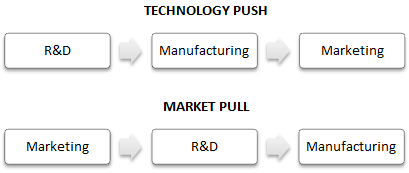
\includegraphics{techno.png}
			\caption{Schematic presentation of technology push and market pull models.}
			\label{fig:models}
		\end{center}
	\end{figure}
	\paragraph{}
	Although it is unlikely to find enterprises that do innovation according to one of these two extremes, it is true that a particular invention derives from an impulse that is closer to one of these two models and subsequently implicates different procedures on the innovator's part, upon which we are not going to enlarge.
	\paragraph{}
When asked about the \emph{tug-of-war} between them, Dr. Erika \textsc{Wagner}, the Executive Director of the X PRIZE Lab@MIT, said \cite{awolfson_entrepreneurship_2010} : \begin{quote}\enquote{Is an entrepreneur with a market need in mind and a product to fit that need better positioned for success than an entrepreneur who starts with a technology but \emph{needs} a need? I'd argue yes.}\end{quote} Indeed, this reasoning is embodied in such start-ups as Hidacs and Future Instruments: whereas Mr. \textsc{Marmaroli} received a direct request to implement a technology, Mr. \textsc{Crevoisier}'s success never came to be because of the lack of initial need expressed by the potential customers. This is the reason why collection of feedbacks during the development phase was not necessary in the first case, but decidedly so in the second one.
	\paragraph{}
	Nowadays, everyone with a good idea and an entrepreneurial proclivity has the possibility of founding an enterprise. For a student there is not even the need to own initial capital, as universities are becoming real launch pads for start-ups in every regard. They are a relatively fail-safe system, with an excellent network of contacts, diversity of ideas and opinions, financial offers, fully equipped laboratories and technical support at disposal \cite{stagars_university_2015}. Instances of this trend are Hidacs and GlobalNeonat: the first was born out of a PhD project in EPFL laboratory, the second saw Mr. \textsc{Rime} conducting the research on the incubator as a master project. In both cases, though, the innovative idea did not originated from them but from the university or its partners (MetaMedia Center). This had also an indirect effect on the technical feasibility. In fact, contrarily to the other two innovators' cases, Mr. \textsc{Marmaroli} and \textsc{Rime} did not have enough practical knowledge at first to embark in such a project without the assistance of professors and colleagues with practical experience in the field. As they both underlined, there was a certain level of uncertainty related to feasibility. For instance, Hidacs is currently composed of four friends that equally share risks and profits, but the technology was developed in a laboratory environment where the regular interaction with experts and individuals from various disciplines provides a fantastic vehicle for innovation. Indeed, there are not many platforms besides the university that provide such an opportunity. These people's contribution was therefore essential not only in the development of the product, but also in providing the technical and practical knowledge, together with the discipline and the work ethic, that is generally lacking in a fresh-faced student but is otherwise needed to launch a start-up. Therefore, if Mr. \textsc{Rime} had to face some major challenges while building the prototype for his incubators, Mr. \textsc{Marmaroli} has been experiencing uncertainty regarding feasibility since the product was marketed, as the clients have different tastes that make customization a requirement, which in turns increases the risk of having a final product that does not work in the way it is supposed to. On the contrary, for Future Instruments and Artanim Interactive it was never a question of feasibility, as they both could benefit from their years-long experience with working outside of the university environment. In their case, once the product is put to market, it is deemed as perfectly working.
	\paragraph{}
	Lastly, it is important to discuss financing. Although it is not directly related to uncertainty, it certainly has a big impact on it as it increases risks. At the initial stage of an enterprise, a lender or an investor do not exist yet, making a personal financial investment the only alternative – unless the innovator is assisted by an institution, such as the university or a foundation. The lack of founding can seriously undermine the development project, as cash is needed to buy raw material, rent facilities, make trips away from home and to pay every kind of external helpers. Furthermore, it is not even sufficient to have an innovative idea, a solid business plan and a working prototype – as Mr. \textsc{Crevoisier}'s experience taught – but a potential investor who is aware of the risks expects the product to be ready to be sold, with a well-defined market segment. This is the reason why, in general, if money is not an issue, the uncertainty regarding an innovation can be significantly decreased.







	%%%%%%%%%%%%%%%%%%%%%%%%%%%%%%%


	\chapter{Description of the start-up}
	\label{ch:description}
	\section{SqeedTime}
	SqeedTime is a new start-up from Lausanne. Its purpose is to provide a smartphone application to enforce the link between local shops, restaurants or all kinds of professionals and the potential customers.
	\paragraph{Organization}
	At first, SqeedTime was founded by Paul-Edgar \textsc{Levy} and Timothée \textsc{Barghouth}, two law students. Now, SqeedTime consists of a team of five members.
	\paragraph{History and original idea}
	During summer 2014, both entrepreneurs observed that even with social networks, they could not organize a spontaneous meeting with friends. Such an inconvenience make them decide to create such a tool, which finally leads to the application soon to be released.
	\section{Application}
	



	\chapter{Uncertainty related to the digital domain}
	\label{ch:kinds}
	\section{The uncertainty in digital innovation field}
	\paragraph{}
	The level of uncertainty depends as much on the product as on the sector it belongs to. As far as the various activity sectors are concerned innovation may be either a necessity, common practice, welcomed or unprecedented.
	\paragraph{}
	In the era of digital convergence, digital content services (services that deliver content created, used, shared, accessed and preserved in a digital format) are highlighted as a driver of innovation \cite{toivonen_innovation_2007, gwee_innovation_2009}. The innovation in this sector does not only transform the existing markets, but creates an opening for new opportunities. This is made possible because of the products' unique characteristics \cite{kim_patterns_2012}:
	\begin{itemize}
		\item digital content services use common digital formats: a network facilitates delivery and share of all kinds of content;
		\item content is edited easily and augmented using multiple available sources (mash-up in web service);
		\item digital content services possess the characteristics of both product and service, so that potential of innovation is increased.
	\end{itemize}
	\section{The case of AppStores, uncertainty of distribution plateforms}
	\paragraph{}
	Recently, what have been highlighted as new content services are mobile applications (apps) in App Stores. Product of this kind have proliferated in the last years. The enormous growth of this sector - coupled with its low market-entry cost for developers and growing list of enviable success stories - attracted the attention of entrepreneurs, to whom Apple's App Store and the Android Market provide easy access \cite{wacheski_anystone_2011}.
	\paragraph{}
	However, the endless possibilities which this sector seems to offer could actually make it only fool's gold, as they increase competition and risk of failure. Among more than one million and a half of apps in the Apple App Store, getting noticed and generating substantial revenues is a great challenge for entrepreneurs, who must aim for innovation if they want to gain success.
	\paragraph{}
	As far as uncertainty is concerned, application developers can face uncertainty related to either market, product or feasibility. 
	\paragraph{}
	Regarding the first one, it is imperative to define a market for one's innovative idea, because a lack of consideration for this issue can result in unquestionable failure. Although it is true that high competition spurs innovation, an entrepreneur should always be aware of the potential customers' needs and wants, especially if his app's concept was born out of his own need and not by observing the other's. Indeed, market uncertainty is probably the one feature that all activities with a commercial goal have in common.
	\paragraph{}
	Despite the similarities in the types of uncertainty concerned, one of the main differences between a physical product and a digital content service is that whereas a manufacturer often handles the direct sale to the customers and can choose the best strategy to cultivate this relationship, an app developer is forced to subject to the platform's rules and constraints. The digital content is delivered from a service provider to the end user by the means of a platform, such as Apple Store, Google Play, etc. (see fig. \ref{fig:content_service}~p.\pageref{fig:content_service}). This means that particular attention should be given to the choice of the store in which one intend to sell its mobile application. For instance, Apple implemented an App Review process to evaluate all submissions and filter them on the basis of some criteria, such as the replication of an already existing application or the expected reaction on the customers' side. Thus, it is evident that a major uncertainty related to the product is present, therefore a developer should be able to define the concept of his product and self-evaluate the willingness to buy it of the customers. Indeed, experiences of various start-ups revealed that the inability of some entrepreneurs to see beyond their enthusiastic confidence in their ideas ultimately brought them to denied entrance in the store and ensuing financial losses. More sensible developers, though, are able to repeatedly evaluate the product concept and their objectives, going through many iterations of trial and error to transform a great idea into a great application, even if the result is not as originally expected. \enquote{It is better to fail fast, learn, and move on quickly}, the CEOs of Anystone Technologies, a mobile applications start-up, commented in this regard.
	\begin{figure}
		\begin{center}
			% Graphic for TeX using PGF
% Title: /home/martin/Documents/EPFL/Master/Semestre I/SHS-1/Rapport_semestre_I/figures/content_service.dia
% Creator: Dia v0.97.3
% CreationDate: Sat Dec 19 00:31:14 2015
% For: martin
% \usepackage{tikz}
% The following commands are not supported in PSTricks at present
% We define them conditionally, so when they are implemented,
% this pgf file will use them.
\ifx\du\undefined
  \newlength{\du}
\fi
\setlength{\du}{15\unitlength}
\begin{tikzpicture}[scale=2]
\pgftransformxscale{1.000000}
\pgftransformyscale{-1.000000}
\definecolor{dialinecolor}{rgb}{0.000000, 0.000000, 0.000000}
\pgfsetstrokecolor{dialinecolor}
\definecolor{dialinecolor}{rgb}{1.000000, 1.000000, 1.000000}
\pgfsetfillcolor{dialinecolor}
\pgfsetlinewidth{0.050000\du}
\pgfsetdash{}{0pt}
\pgfsetdash{}{0pt}
\pgfsetmiterjoin
\definecolor{dialinecolor}{rgb}{0.000000, 0.000000, 0.000000}
\pgfsetstrokecolor{dialinecolor}
\draw (33.000000\du,11.000000\du)--(33.000000\du,16.000000\du)--(39.000000\du,16.000000\du)--(39.000000\du,11.000000\du)--cycle;
% setfont left to latex
\definecolor{dialinecolor}{rgb}{0.000000, 0.000000, 0.000000}
\pgfsetstrokecolor{dialinecolor}
\node[anchor=south west] at (33.000000\du,11.000000\du){Digital content};
\pgfsetlinewidth{0.050000\du}
\pgfsetdash{}{0pt}
\pgfsetdash{}{0pt}
\pgfsetmiterjoin
\definecolor{dialinecolor}{rgb}{0.000000, 0.000000, 0.000000}
\pgfsetstrokecolor{dialinecolor}
\draw (33.400000\du,14.600000\du)--(33.400000\du,15.600000\du)--(38.600000\du,15.600000\du)--(38.600000\du,14.600000\du)--cycle;
% setfont left to latex
\definecolor{dialinecolor}{rgb}{0.000000, 0.000000, 0.000000}
\pgfsetstrokecolor{dialinecolor}
\node at (36.000000\du,15.10000\du){Platform};
\pgfsetlinewidth{0.050000\du}
\pgfsetdash{}{0pt}
\pgfsetdash{}{0pt}
\pgfsetmiterjoin
\definecolor{dialinecolor}{rgb}{0.000000, 0.000000, 0.000000}
\pgfsetstrokecolor{dialinecolor}
\draw (33.400000\du,11.600000\du)--(33.400000\du,13.600000\du)--(38.600000\du,13.600000\du)--(38.600000\du,11.600000\du)--cycle;
% setfont left to latex
\definecolor{dialinecolor}{rgb}{0.000000, 0.000000, 0.000000}
\pgfsetstrokecolor{dialinecolor}
\node[anchor=south west] at (33.400000\du,11.600000\du){Content};
\pgfsetlinewidth{0.050000\du}
\pgfsetdash{}{0pt}
\pgfsetdash{}{0pt}
\definecolor{dialinecolor}{rgb}{0.000000, 0.000000, 0.000000}
\pgfsetstrokecolor{dialinecolor}
\pgfpathellipse{\pgfpoint{34.800000\du}{12.600000\du}}{\pgfpoint{1.000000\du}{0\du}}{\pgfpoint{0\du}{0.600000\du}}
\pgfusepath{stroke}
% setfont left to latex
\definecolor{dialinecolor}{rgb}{0.000000, 0.000000, 0.000000}
\pgfsetstrokecolor{dialinecolor}
\node at (34.800000\du,12.600000\du){Product};
\pgfsetlinewidth{0.050000\du}
\pgfsetdash{}{0pt}
\pgfsetdash{}{0pt}
\definecolor{dialinecolor}{rgb}{0.000000, 0.000000, 0.000000}
\pgfsetstrokecolor{dialinecolor}
\pgfpathellipse{\pgfpoint{37.200000\du}{12.600000\du}}{\pgfpoint{1.000000\du}{0\du}}{\pgfpoint{0\du}{0.600000\du}}
\pgfusepath{stroke}
% setfont left to latex
\definecolor{dialinecolor}{rgb}{0.000000, 0.000000, 0.000000}
\pgfsetstrokecolor{dialinecolor}
\node at (37.200000\du,12.600000\du){Process};
\pgfsetlinewidth{0.050000\du}
\pgfsetdash{}{0pt}
\pgfsetdash{}{0pt}
\pgfsetbuttcap
{
\definecolor{dialinecolor}{rgb}{0.000000, 0.000000, 0.000000}
\pgfsetfillcolor{dialinecolor}
% was here!!!
\pgfsetarrowsend{stealth}
\definecolor{dialinecolor}{rgb}{0.000000, 0.000000, 0.000000}
\pgfsetstrokecolor{dialinecolor}
\draw (36.000000\du,13.600000\du)--(36.000000\du,14.600000\du);
}
\pgfsetlinewidth{0.050000\du}
\pgfsetdash{}{0pt}
\pgfsetdash{}{0pt}
\pgfsetbuttcap
{
\definecolor{dialinecolor}{rgb}{0.000000, 0.000000, 0.000000}
\pgfsetfillcolor{dialinecolor}
% was here!!!
\pgfsetarrowsend{stealth}
\definecolor{dialinecolor}{rgb}{0.000000, 0.000000, 0.000000}
\pgfsetstrokecolor{dialinecolor}
\draw (35.800000\du,15.600000\du)--(35.800000\du,17.600000\du);
}
\pgfsetlinewidth{0.050000\du}
\pgfsetdash{}{0pt}
\pgfsetdash{}{0pt}
\pgfsetbuttcap
{
\definecolor{dialinecolor}{rgb}{0.000000, 0.000000, 0.000000}
\pgfsetfillcolor{dialinecolor}
% was here!!!
\pgfsetarrowsend{stealth}
\definecolor{dialinecolor}{rgb}{0.000000, 0.000000, 0.000000}
\pgfsetstrokecolor{dialinecolor}
\draw (36.200000\du,17.600000\du)--(36.200000\du,15.600000\du);
}
% setfont left to latex
\definecolor{dialinecolor}{rgb}{0.000000, 0.000000, 0.000000}
\pgfsetstrokecolor{dialinecolor}
\node[anchor=north] at (36.000000\du,17.600000\du){User};
\end{tikzpicture}

			\caption{Structure and components of digital content services (\cite{kim_patterns_2012})}
			\label{fig:content_service}
		\end{center}
	\end{figure}
	\paragraph{}
	As for minimizing risks inherent development and feasibility, \cite{tiwana_platform_2014} suggests to schedule stages with the greatest uncertainty as late as possible in the project roadmap. Unless there is a clear first-mover advantage, at first a developer should focus on opportunities with the least technical uncertainty and the highest immediate payoff, ensuring that the benefits will begin being collected earlier rather than later. This approach can reduce challenges as well as uncertainty in the subsequent stages, as new information – regarding the market, the customers' issues and needs, further developments, etc. – can be obtained during the implementation of the preceding stages. Even if some steps of the future strategy might be never executed, at least some payoff is generated from what is feasible instead of pursuing an all-or-nothing proposition.
	\paragraph{}
	Analyzing the experiences of other start-ups in this sector, we can point out some of the most important aspects which an app developer should keep into account if he wants to transition into the market as smooth as possible:
	\begin{itemize}
		\item \emph{App stores' differences:} the main app stores nowadays are Apple App Store, Google Play (Android), BlackBerry App World and Windows Phone App Marketplace. Each one of them has different characteristics that may suit an entrepreneur better or worse. For instance, with respect to the majorly used ones, the advantage of Google Play is the wide choice it offers and its open source model, enabling nearly anyone to add their apps. However, Android suffers from the drawback of running on many hardware platforms, which forces the developers to cover multiple designs and testing permutations. In contrast, there is a greater guarantee of quality in the Apple Store than with Android, as Apple tests and approves every app that goes on sale in the App Store. Furthermore, the exclusivity of the Apple system limits the hardware variants tremendously. This contributes to Apple Store's popularity among the mobile users, making it the most profitable for developers – if not the best choice. In addition, while Google Play allows the developers to be in direct contact with the customers and provides them with some detailed statistics about users, the Apple Store does not allow anything of all this.
		\item \emph{Predominant sales model in the app store:} although an entrepreneur would like the option to choose whether his app should be available for free or for a price, he should also consider which is the predominant sales model in the chosen app store. In fact, despite the willingness of consumers to pay for a useful mobile application, if the app store encourages the sellers to include a free or \emph{lite} edition of their products with limited capabilities, this trend should not be overlooked. Consumers are reluctant to pay for an application without trying it first and making it free removes a powerful mental barrier from potential purchases, increasing revenues.
		\item \emph{Price changes and promotions:} they can greatly influence download rates and sales. They become advertisement tools when there are mobile applications that monitor price drops, and should be used to prompt more reviews online and by word of mouth. Time-limited promotions are also particularly useful when the product includes a free version besides the full one. This makes advertising mostly unnecessary as the free edition's goal is already to encourage the purchase of the complete edition. Nonetheless, purchasing behavior should be well monitored to keep track of the products' sales.
		\item \emph{Customers' reviews:} they are a powerful tool that can impact on sales (positively or negatively), revenues and advertising costs. As much as it is rewarding to receive high grades from customers, complaints should not be overlooked because they can dissuade purchases, especially in a highly competitive environment such as the mobile applications’ one. Therefore, it is imperative that the product development is never discontinued to offer regular upgrades and avoid and/or resolve issues that are pointed out by customers.
	\end{itemize}

	\chapter{Working methodology}
	\label{ch:method}
	\section{Objectives and general approaches}
	\paragraph{Introduction }During the second semester, our goal is to observe the start-up SqeedTime, to highlight some correlations between some signals, some events or tendencies. We will have two approaches of this problem, two methodologies, based on what we what to observe. Based on chapter \ref{ch:kinds}, we will proceed with a comparison with other start-ups belonging to the same domain.

	\paragraph{Precise observation}Our first approach is to make some hypotheses on which signals could be correlated or not, and to gather precise data to verify them. This approach requires two steps : 
	\begin{itemize}
		\item We have to be able to formulate precise and simple enough hypotheses. Making too general or too complex hypotheses would lead not to search for specific behavior, leading to the failure of the verification. This approach does not aim for an exhaustive model of correlations\footnote{If specialists of the field still encounter difficulties, it is definitivelly not possible for us, in such a short amount of time and of knowledge.}.
		\item Once these points are well defined, we then have to develop specific tools to evaluate the signals. Here, the goal is to develop an high-level framework for data analysis, i.e. to guess which metrics would be significant for the evaluation, then to work on a way to compute this metric, and finally to have a relevant way to measure the data needed for these calculations.
	\end{itemize}
	We want to highlight the fact that this approach is uncertain. Even if it is possible to make good hypotheses, which then appears to be relevant with time, it is possible that this approach will lead to a complete fail as well. Also, even if the developped framework appears to be significant in our case, one should test it with other start-ups to verify its relevance. This approach requires an high amount of work before starting the actual observation, but afterwards it only entails data collection and verification or invalidation the hypotheses.
	\paragraph{General observation}Our second approach is the exact opposite of the first one. This time, we observe the startup as an external viewer, i.d. we consider the startup globally. After observing the whole startup for a given amount of time, we try to catch relevant events, and finally to identify their causes. This approach does not focus on events \emph{a priori} ; we will have global tendencies for events, but we will not focus on a single event, or on single cause. It is like applying reverse engineering to the uncertainty problem. 
	\begin{itemize}
		\item At first, we have to define which data we want to collect, at which rate, etc. The more types of and the more fined-grained the data, the more precise will be the analysis, but the harder to collect, store, and analyse. We have to make a compomise with these different parameters.
		\item Once our data set is collected, we have to execute a huge analysis. For this approach, we will have to develop the relevant tools \emph{a posteriori}. 
	\end{itemize}
	This approach needs good heuristics on the parameters of data collection, since it is clearly not possible to get all the information. Making heuristics may lead to holes in the data fabric we are building. These hole may be filled by gathering wide enough events, at the cost of not being able to detect smallest causes.

	This approach requires an high amount of work after the data collection to understand the causality processus which occured during the observation.
	\section{First method}
	\label{ch:first_method}
	The first method allows us to verify precise hypotheses. The high degree of accuracy that we want to achieve coupled with somewhat generalized hypotheses inevitably lead to the collection of a great amount of data. To avoid this we should take care into structuring a formulation as tapered as possible. Nevertheless, such a method provides us with strong results. 
	\subsection{Hypothesis}
	In our case, examples of hypotheses could be :
	\begin{quote}{H1 : }
		The number of new subscribers per week decreases due to the exam session
	\end{quote}
	\begin{quote}{H2 : }
		We can observe the effect of an exam session on the number of new subscribers after $x$ weeks.
	\end{quote}
	At this point, hypotheses sould be as clear as possible from an external point of view. In particular, it is useful to keep it in natural language, so non-specialists (as the actors in the startup) can understand it and exploit the forthcoming results as a blackbox.
	\subsection{Metrics}
	The second part consists in describing which metrics are relevant. To achieve that, we should formalize the problem. If we keep the previous examples, we want to verify the following :
	$$E \Rightarrow \exists t > t_e : N(t) < N(t_e) - N(t_{th})$$
	$$\Delta_t = x,\ \Delta_t = t_d - t_e$$
	With $E$ being the statement \emph{The actors have an exam session}, $t_e$ being the beginning of the exam session and $t_d$ being the first time after $t_e$ such that $N(t_d) < N(t_e) - N_{th}$, $N(t)$ being the number of new subscriber the week before $t$ and $N_{th}$ a significant threshold.
	After formalizing the hypotheses, it is easy to have the metrics we are interested in. For instance, in our case it can be $N_{th}$, $x$, etc.
	\subsection{Analysis}
	Once with the formal model developped, we can also work on the analysis we have to do. For instance, in both previous cases, a possibility is a rolling average of $N(t)$ over one week, for $t$ going from $t_e$ to $t_{max}$ (a given parameter, time after which we suppose the exam session is not relevant anymore), with a step of $\delta_t$ (another parameter). The result of the analysis would be \emph{true} or \emph{false} for H1, and $x$ for H2 (in case H1 is \emph{true}, H2 makes no sense otherwise). 
	\subsection{Data requirements}
	Finally, once our analysis method is developped, we finally know which data to look for, and at which sampling rate. The actual observation can start. For instance, in our case we need to make a rolling average. The rolling average ($A(t, \delta_t) = \frac{\sum_t^{t + \delta_t}n(t)}{\delta_t}$, $n(t)$ being the number of new subscriber at day $t$) can be either measured, by asking everyday the previous week results, or by asking everyday the previous day result. The question is what is feasible ? What is better ? Maybe the startup already has the week result. The idea is to ask them for the least expansive data, not to modify their behavior.

	\section{Second method}
	This method is based on a wide (and kind of random) observation. The idea is to gather as much data as our data storage allows us. After that we use statistical methods to analyse these observations, such as \emph{k-mean} or other machine-learning algorithms, to actually get trends. In that method, the principal constraint is the actual quantity and quality (precision) of data we can have. As we see below, one has to make a compromise between these parameters and the time he wants to spend on computations.
	\subsection{Evaluation of our limits}
	\paragraph{}
	At first, it is required to establish a limit on how much data we can gather. These limits can be physical (such as data storage limit, computation time allowed), legislation (\enquote{What am I allowed to gather ?}), the way to collect data (\enquote{I can only collect data via paper form}), or any other type. This first step will obviously restrict our data set. At this point, we are forced to make hypothesis on the subject, as it is our source of data (whether it actively provides them or not) and we don't want to modify its behavior.
	\paragraph{}
	For instance, given that we estimate our computation time at $C\times S_d$ ($C$ a coefficient, $S_d$ the size of the dataset), and that the subject can provide $S_p$ (size of data provided per day) for $\delta_t$ days. The size of the dataset is $S_d = S\times N_S\times D$ ($C$ a coefficient, $S$ the size of each sample of each dimension, $N_S$ the number of samples, $D$ the number of dimensions of the dataset). Knowing that we can obtain at most $S_p\times \delta_t$ data, we have the constraint $ S\times N_S\times D\leq S_p\times \delta_t$. Then we have to make a compromise between precision (i.e. size of the sample), number of source events (i.e. number of dimensions we observe) and the granularity of our results (i.e. sampling rate).
	\subsection{Data type}
	\paragraph{}
	As we don't know the final observation we want to do, we want our data to be as spread out as possible, so they cover the widest events. We have two degrees of freedom we can play with. The first is the accuracy (i.e. which precision we want on a given dimension of our dataset space). The second is correlation between dimensions and the number of dimensions. 
	\paragraph{}
	The first can be tweaked depending on which the accuracy of the result we hope for, knowing that the size of the dataset decreases logarithmically with the loss of precision (halving the precision result on a constant decrease on the size of the dataset). One should be aware of such a relation between precision and size. As it may be interesting not to focus on too precise data, reducing precision become expensive quite fast (the lost of precision is exponential w.r.t the decrease of the dataset size).
	\paragraph{}
	The second parameter is the number of independent dimensions. The problem is that we don't know the correlation between these axis, since it is exactly the kind of relation we want to extract from these. The idea is then to make heuristics on wich data we sample. Here, the more the data are independant, the more space they require (linear relation) from the definition of the mutual entropy $H(x,y) = H(x)+H(y|x)$, and knowing that the dataset size is proportional to the entropy. The consequence is that it requires less space to store dependant data than independant one (assuming we achieve a perfect compression). But getting related data is not what we are interested in in this method, since we want to catch the maximum of different signals. Hence, we have (assuming that our heuristics are good and provide us independant data) to make a compromise between \emph{coverage} of our dataset and its size.
	\paragraph{}
	Fig.~\ref{fig:tradeoff} p.~\pageref{fig:tradeoff} represent the tradeoff one has to face.
	\begin{figure}
		\begin{center}
			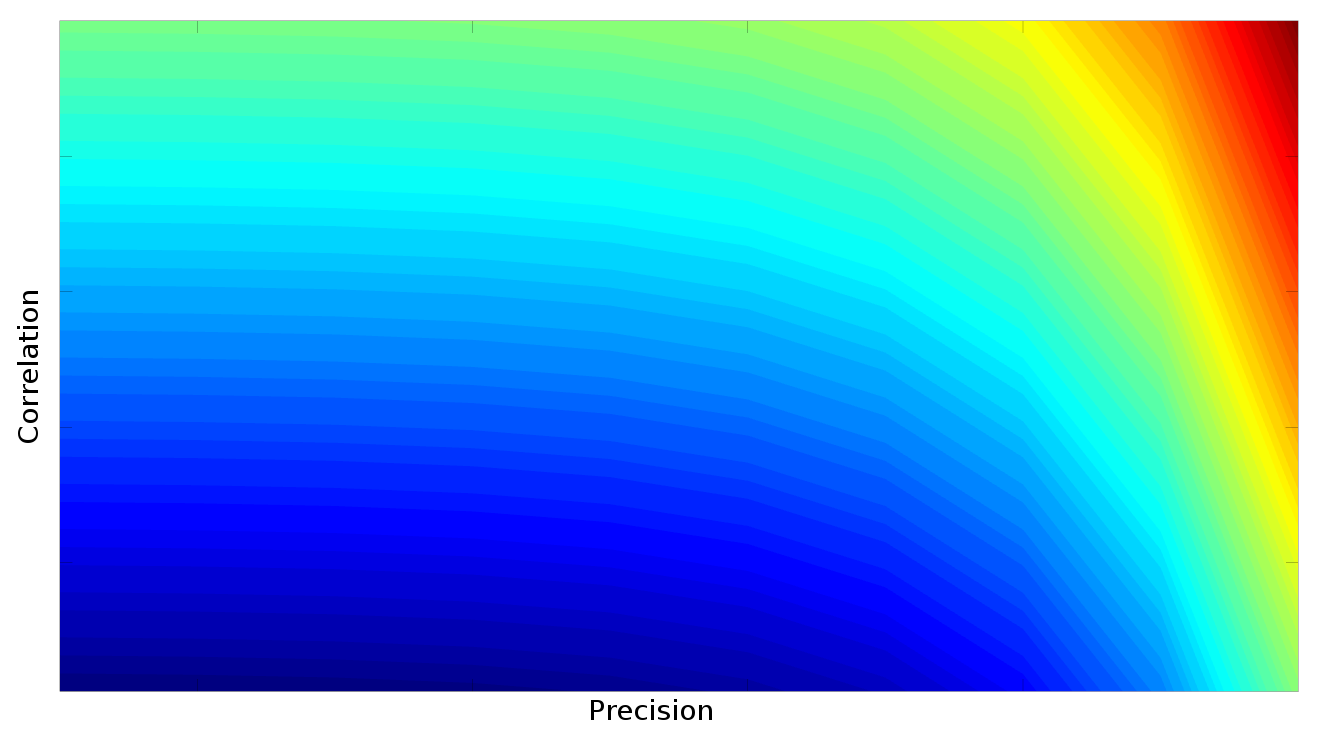
\includegraphics[width=\textwidth]{tradeoff_m2.png}
			\caption{Tradeoff between precision ($x$-axis) and correlation ($y$-axis)}
			\label{fig:tradeoff}
		\end{center}
	\end{figure}
	\subsection{Sampling rate}
	\paragraph{}
	The sampling rate is a tricky part, because it is directly related to the time frequency of the smallest data we can extract from the dataset. As the \textsc{Nyquist}-\textsc{Shannon} sampling theorem states, the sampling frequency is twice the frequency of the smallest signal that you can gather.
	\paragraph{}
	Also, the size of the dataset increases linearly w.r.t the sampling frequency. So one has to take a sampling rate to be able to extract representative information, but keeping in mind that the dataset (and then probably the computation time) will increase.
	\section{Procedure for data collection}
	\subsection{Face-to-face meeting}
	\paragraph{}
	After formalizing the methods to collect and analyze data, we need to face the question of how to collect the required information. In this regard, we plan to proceed with both face-to-face meetings and written queries. 
	\paragraph{}
	Time permitting on the start-ups members’ side, the meetings will take place at regular intervals, allowing for a decreasing frequency over time, as everyone will have developed a general understanding on what the monitoring activity entails. The upfront contacts are fundamental in gathering specifics about the company’s developments and other approaches could not be as effective.
	\paragraph{}
	For instance, it would be impossible to know the amount of oral confrontations between the members of the team. Also, we should develop a kind of operational procedure on \emph{how to} collect this information : how to measure it? Which signs should be taken into account ? etc. with respect to the relevant signals defined in the working methodology (cf. chapter \ref{ch:method}).
	\subsection{Survey}
	\paragraph{}
	To compensate for the physical impossibility of meeting as many times as we wish due to obvious commitments on both sides (ours and the company’s members’), we have thought to forward a survey with a series of quickly answerable questions to the start-up components. It will be prepared in advance and provided to them so that they can fill it with a certain regularity, without fearing of it taking away too much of their time, since the majority of the questions will be structured as multiple choice or in a similar way.
	\paragraph{}
	The survey is intended for both the founders and the software developers, as we estimate that their points of view are going to be substantially different in some respects and must therefore be taken into account. The topics will cover two areas of interest: business-administrative matters and development. Thus, for instance, the developers will be asked to record the number of hours of work per week and what they deem necessary to do in the future, whereas the founders will be aware of valuable data such as sales, number of active users and unsubscriptions, number of new restaurants that agreed to a partnership and their feedback on the service received thanks to the smartphone application, as well as the number of restaurants that revoked the affiliation, the frequency and nature of users’ complaints, the regularity of software updates, new costs in which they incurred, etc. For the majority of the mentioned topics, an approximate estimation of future results will be requested from the start-up component. The reason lies behind our belief that incertitude also derives from the innovators’ misguided expectations, since an overly optimistic or pessimistic mindset on the future trends will have a significant impact on how they execute daily activities and perceive risks. This very impact will be evaluated through a comparison of the two datasets – procrastinated and measured.
	\paragraph{}
	It is particularly important that the company’s members specify the milestones (both administrative and concerning development) that they want to reach at every step of the product development and that they estimate at which point they are on the path to achieve them every time they fill the form. This will help us in discerning the pace that the start-up is adopting, and to compare the data over different time slots, for instance between a period of fervent work and one in which exams are the only preoccupation for the team.
	\paragraph{}
	Lastly, we feel that a personal note needs to be included, i.d. a query on the member’s degree of satisfaction of their work and the company’s results. Even if not objective and apparently ineffectual, this inquiry constitutes relevant data in light of the fact that motivation drives innovation. Indeed, it is a concept on which all the four guests in the first semester remarked. If for some reasons the components of an enterprise start showing a lack of interest in what they are doing, it is only logical that the company will show the brunt of it: the product will not be regularly or appropriately updated and advertised, the number of customers and partners will go stale or decrease. Clearly, a lack of motivation can be both the consequence or the driver of bad results, therefore it is certainly interesting to analyze how this could correlate with the performance of the company.
	\subsection{Gantt Chart}
	\begin{landscape}
		\begin{figure}
			\begin{center}
				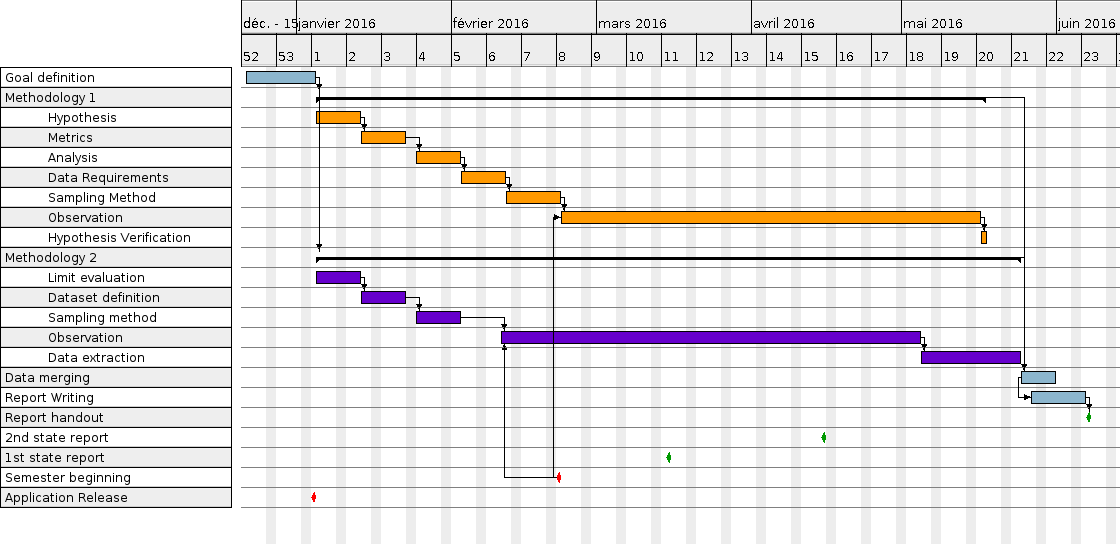
\includegraphics[width=1.5\textheight]{../Gantt/Planning.png}
				\caption{Gantt chart of the \nth{2} semester}
				\label{fig:gantt}
			\end{center}
		\end{figure}
	\end{landscape}
	\paragraph{}
	Once the activities for next semester have been defined, it is possible to display them in a Gantt diagram (see fig.~\ref{fig:gantt} p.~\pageref{fig:gantt}). Its purpose is to estimate the actual length of the flanking process, by sequencing the steps and summing their individual durations. At the end of the semester we will thus be able to compare our plan with what actually occurred and derive conclusions on our overall performance.
	\paragraph{}
	As above-mentioned, the working methodology consists of two methods that have to be implemented in parallel. For both of them, the first step requires the definition of our objectives, without which we would be actually proceeding with blindfolded eyes.
	\paragraph{}
	As far as the first methodology is concerned, section \ref{ch:first_method} already suggests the sequence of the initial activities, i.d. delineation of the hypotheses, the metrics, followed by the analysis and the outlining of the data requirements. In an analogous manner, the second method entails the evaluation of our limits and the dataset definition. The observation period will be quite extensive, as it will provide data from which we will extract all the relevant information. One can observe that by developing two approaches of this kind we achieve a synergy, which originates from the fact that the first method implies a bigger effort at the beginning of the semester, the second one at the end.
	\paragraph{}
	Once we will be satisfied with the amount of material collected, we will proceed with the merging of the data, which will result into a comprehensive analysis that will be illustrated in the final report.





	\chapter*{Conclusion}
	\paragraph{}
	The aim of this report was to describe how we can analyze the level of uncertainty in a start-up that belongs to the activity sector of mobile applications. 
	\paragraph{}
	The bases on which we found our research are described in chapter \ref{ch:knowledge}, which summarizes the observations we made as a class on the experiences of four different start-ups (Hidacs, Future Instruments, GlobalNeonat, Artanim Interactive). As their cases highlight different facets of uncertainty in enterprises that are going through the early stage of their life cycle, we have been able to build knowledge on this topic, on the means to identify it, categorize it and use it to determine weaknesses and recommendations. We intend to apply this very sequence to SqeedTime, a newly founded start-up based in Lausanne that provided a smartphone application to enforce the link between local shops, restaurants and the customers. 

	In chapter \ref{ch:description}, we describe its product, organization and all characteristics of a certain relevance for our purposes, with a particular emphasis on the definition of the activity sector, to which the entire chapter \ref{ch:kinds} is dedicated. 
	
	Indeed, we realized that most start-ups share the types of risks with others that specialize in the same business. Mobile applications, and in general digital content services, represents one of the sectors with the greatest potential for innovations, as they combine product with service and are easily created, edited and used. However, this same potential increases competition, which in turn enlarges risks. Therefore, it is conducive to our purposes to analyze the industry and consider similar start-ups’ experiences. We use this analysis to execute a preliminary estimation of the incertitude related to SqeedTime. 
	
	We conclude the article with the major topic that is also the purpose of this report and the first step and groundwork for the project of next semester: the working methodology. What we were able to learn so far provide us with the means to formulate a plan for next semester that should allow us to flank the start-up in a coherent way and to gather significative knowledge. Our objective is to highlight some correlations between signals, events or tendencies, which will be useful information not only to define the level of incertitude, but also to verify how the start-up members’ personal projection of the future compares to the actual results. We determined that we can employ two approaches: the first one originates by our intention to verify some initial hypotheses, for the purpose of which we evaluate the possible methodology and the subsequent data that is needed; the second one aims to collect general data on the company that will be eventually used at a later stage to make more assumptions on the level of incertitude. The data will be collected through periodic face-to-face meetings with the members and a fillable form with a series of standard questions that they will answer. It will be formulated in a manner that will not take much time away from them and will still be an useful tool to compensate for the lack of direct contact, which will be inevitably constrained by the student activities required of the founders.
	\paragraph{}
	Lastly, we would like to draw the attention to the fact that both working methodology and incertitude vary greatly depending on the stage at which the enterprise finds itself. In our case, SqeedTime has not existed for long and the smartphone application will be launched soon. Hence, as the customers’ response is still lacking, uncertainty is currently at its peak level and a hectic development phase will follow should the products show promising results. The working methodology that we formulated takes all this into account and has been planned in a way that should allow us to gather the most relevant information at a stage where the members of the start-up will undertake serious actions to improve their smartphones application – as and if it will show a certain measure of market acceptance.
	\appendix
	\bibliographystyle{alpha}
	\bibliography{SHS}
	\end{document}
